% Revisi\'on Sistem\'atica de Literatura - Metodolog\'ia Kitchenham
% Inteligencia Artificial Aplicada al Desarrollo de Software en Contextos Empresariales
% Universidad de las Fuerzas Armadas ESPE - Ingenier\'ia en Software
%
\documentclass[runningheads]{llncs}
%
\usepackage[T1]{fontenc}
\usepackage{graphicx}
\usepackage[utf8]{inputenc}
\usepackage[spanish]{babel}
\usepackage{booktabs}
\usepackage{multirow}
\usepackage{hyperref}
\usepackage{xcolor}
\usepackage{array}
\usepackage{float}
\usepackage{tabularx}

% Configuracion de hyperref
\hypersetup{
    colorlinks=true,
    linkcolor=blue,
    citecolor=blue,
    urlcolor=blue
}

%
\begin{document}
%
\title{Inteligencia Artificial Aplicada al Desarrollo de Software en Contextos Empresariales: Una Revisi\'on Sistem\'atica de Literatura}
%
\titlerunning{IA en Desarrollo de Software Empresarial}
%
\author{Mesias Orlando Mariscal O\~{n}a\inst{1} \and
Denise Noemi Rea Diaz\inst{1} \and
Julio Enrique Viche Castillo\inst{1}}
%
\authorrunning{ }
%
\institute{Carrera de Ingenier\'ia en Software,\\
Universidad de las Fuerzas Armadas ESPE, Ecuador\\
\email{\{momariscal, dnrea, jeviche\}@espe.edu.ec}}
%
\maketitle
%
\begin{abstract}
Esta revisi\'on sistem\'atica examina la adopci\'on de Inteligencia Artificial y Machine Learning en el desarrollo de software empresarial siguiendo la metodolog\'ia de Kitchenham y las directrices PRISMA. A partir de una b\'usqueda exhaustiva en IEEE Xplore (368), Scopus (1,012) y SpringerLink (17), se identificaron 1,397 art\'iculos publicados entre 2023-2025. Tras un proceso riguroso de screening y evaluaci\'on de calidad mediante QATQS+CASP, 37 estudios de alta calidad (score 9-12) fueron seleccionados para s\'intesis cualitativa.

Los resultados revelan que ChatGPT (28\%) y GitHub Copilot (24\%) son las herramientas predominantes, mientras que las t\'ecnicas ML/DL tradicionales representan el 34\% de adopci\'on. Los factores de \'exito identificados incluyen automatizaci\'on de tareas repetitivas (n=18), interfaces intuitivas (n=14), e integraci\'on con CI/CD (n=11). Las barreras principales son gesti\'on de expectativas infladas (56.8\%), calidad de datos (54.1\%), falsos positivos (51.4\%), y alucinaciones de LLMs (48.6\%).

Las competencias emergentes clave incluyen prompt engineering (n=16), evaluaci\'on cr\'itica de outputs (n=15), y fundamentos de ML (n=14). Se identificaron pr\'acticas innovadoras como AI-Augmented Development (n=18), RAG-based assistants (n=12), y fairness-aware ML (n=11). El an\'alisis comparativo SME vs. corporaciones revela diferencias significativas: las SMEs prefieren herramientas comerciales (ChatGPT 67\%, Copilot 44\%) por bajo costo, mientras las corporaciones desarrollan LLMs customizados con RAG (57\%).

Se propone un marco tridimensional (tecnol\'ogico-organizacional-humano) para guiar la adopci\'on efectiva, con un roadmap de tres fases. La principal conclusi\'on es que, aunque la adopci\'on individual es alta (75\%), la integraci\'on organizacional permanece limitada, requiriendo un enfoque hol\'istico que equilibre tecnolog\'ia, cultura organizacional y desarrollo de competencias.

\keywords{Inteligencia Artificial \and Machine Learning \and Desarrollo de Software \and Contextos Empresariales \and Revisi\'on Sistem\'atica}
\end{abstract}

%
\section{Introducci\'on}

La Inteligencia Artificial (IA) y el Machine Learning (ML) est\'an transformando fundamentalmente la ingenier\'ia de software. Herramientas como ChatGPT y GitHub Copilot prometen incrementos de productividad de hasta 55\%~\cite{github2024}, pero la evidencia emp\'irica revela brechas significativas entre las expectativas y la realidad organizacional~\cite{kemell2025,dolata2024}. Mientras el 75\% de los desarrolladores utilizan IA de manera individual, la integraci\'on a nivel organizacional permanece limitada por m\'ultiples factores~\cite{jensen2025}.

La revoluci\'on de la IA generativa, iniciada con el lanzamiento p\'ublico de ChatGPT en noviembre de 2022, ha generado un inter\'es sin precedentes en la automatizaci\'on del desarrollo de software. GitHub Copilot, lanzado comercialmente en 2022, report\'o m\'as de un mill\'on de usuarios pagos en su primer a\~no~\cite{github2024}. Sin embargo, esta r\'apida adopci\'on ha generado preguntas fundamentales sobre c\'omo integrar efectivamente estas tecnolog\'ias en contextos empresariales reales.

\subsection{Problema y Gap de Investigaci\'on}

La literatura actual presenta fragmentaci\'on en el conocimiento sobre adopci\'on de IA/ML en desarrollo de software empresarial. Estudios existentes se enfocan principalmente en evaluaciones t\'ecnicas de herramientas espec\'ificas, sin abordar sistem\'aticamente los factores organizacionales, las competencias requeridas, ni las pr\'acticas emergentes que facilitan o dificultan la adopci\'on efectiva.

Espec\'ificamente, se identifican los siguientes gaps: (1) ausencia de s\'intesis sistem\'atica de evidencia emp\'irica reciente (2023-2025), (2) falta de marcos conceptuales que integren dimensiones t\'ecnicas, organizacionales y humanas, (3) escasez de an\'alisis comparativos entre diferentes contextos organizacionales (SMEs vs. corporaciones), y (4) limitada comprensi\'on de las competencias emergentes requeridas para la adopci\'on efectiva.

\subsection{Preguntas de Investigaci\'on}

Esta RSL aborda cinco preguntas de investigaci\'on derivadas de los gaps identificados:

\begin{itemize}
    \item \textbf{RQ1:} ¿Qu\'e herramientas de IA/ML se adoptan en desarrollo de software empresarial?
    \item \textbf{RQ2:} ¿Cu\'ales son los factores de \'exito para la adopci\'on?
    \item \textbf{RQ3:} ¿Cu\'ales son las barreras principales?
    \item \textbf{RQ4:} ¿Qu\'e competencias emergentes se requieren?
    \item \textbf{RQ5:} ¿Qu\'e pr\'acticas innovadoras est\'an surgiendo?
\end{itemize}

Estas preguntas fueron formuladas siguiendo el framework PICOC (Population, Intervention, Comparison, Outcome, Context) adaptado para revisi\'on de literatura en ingenier\'ia de software.

\subsection{Contribuciones}

Este trabajo contribuye con: (1) s\'intesis de 37 estudios de alta calidad metodol\'ogica, (2) marco tridimensional de adopci\'on que integra factores tecnol\'ogicos, organizacionales y humanos, (3) taxonom\'ia de herramientas IA/ML en desarrollo de software, (4) an\'alisis comparativo detallado SMEs vs. corporaciones, y (5) recomendaciones pr\'acticas con roadmap de implementaci\'on en tres fases.

\section{Metodolog\'ia}

Esta RSL sigue las directrices de Kitchenham~\cite{kitchenham2007} y el protocolo PRISMA para asegurar rigor metodol\'ogico y reproducibilidad. El protocolo fue registrado previamente y validado por pares acad\'emicos antes de su ejecuci\'on.

\subsection{Protocolo de Investigaci\'on}

El protocolo incluy\'o cinco fases: (1) definici\'on de preguntas de investigaci\'on utilizando PICOC, (2) estrategia de b\'usqueda sistem\'atica con cadenas validadas, (3) criterios de selecci\'on expl\'icitos con doble revisi\'on, (4) evaluaci\'on de calidad QATQS+CASP con calibraci\'on inter-evaluador, y (5) s\'intesis narrativa estructurada con codificaci\'on tem\'atica inductiva.

La selecci\'on de bases de datos se bas\'o en cobertura de literatura de ingenier\'ia de software: IEEE Xplore (principal fuente de conferencias y journals IEEE), Scopus (mayor \'indice multidisciplinario con fuerte cobertura de ciencias de la computaci\'on), y SpringerLink (publicaciones Springer y LNCS). Esta combinaci\'on maximiza recall mientras mantiene precisi\'on en el dominio.

\subsection{Estrategia de B\'usqueda}

Se realizaron b\'usquedas en tres bases de datos durante noviembre-diciembre 2024. La cadena de b\'usqueda fue desarrollada iterativamente, comenzando con t\'erminos clave y refinando mediante an\'alisis de art\'iculos semilla.

\begin{table}[H]
\centering
\small
\caption{Resultados de b\'usqueda por base de datos}
\label{tab:busqueda}
\begin{tabular}{@{}lrrr@{}}
\toprule
\textbf{Base de Datos} & \textbf{Encontrados} & \textbf{Filtrados} & \textbf{2023-2025} \\
\midrule
IEEE Xplore & 368 & 29 & 22 \\
Scopus & 1,012 & 98 & 66 \\
SpringerLink & 17 & 1 & N/A \\
\midrule
\textbf{Total} & \textbf{1,397} & \textbf{128} & \textbf{88} \\
\bottomrule
\end{tabular}
\end{table}

La cadena de b\'usqueda final combin\'o t\'erminos en tres grupos conceptuales: (1) tecnolog\'ia: ``generative AI'' OR ``large language model'' OR LLM OR ChatGPT OR Copilot OR ``machine learning''; (2) dominio: ``software engineering'' OR ``software development''; (3) fen\'omeno: adopt* OR implement* OR skill* OR practice* OR barrier*. Los grupos se conectaron con operador AND.

\subsection{Criterios de Selecci\'on}

\textbf{Criterios de Inclusi\'on:}
\begin{itemize}
    \item Art\'iculos publicados entre 2023-2025
    \item Datos emp\'iricos primarios (surveys, experimentos, casos de estudio)
    \item Contexto organizacional de desarrollo de software
    \item Menci\'on expl\'icita de herramientas o t\'ecnicas de IA/ML
    \item Enfoque en adopci\'on, competencias, pr\'acticas o barreras
\end{itemize}

\textbf{Criterios de Exclusi\'on:}
\begin{itemize}
    \item Reviews secundarios sin datos primarios propios
    \item Art\'iculos puramente t\'ecnicos sin contexto organizacional
    \item Estudios cortos ($<$4 p\'aginas) o extended abstracts
    \item Duplicados entre bases de datos
    \item Literatura gris sin proceso de peer review
\end{itemize}

\subsection{Evaluaci\'on de Calidad}

Se utiliz\'o una herramienta adaptada de QATQS (Quality Assessment Tool for Quantitative Studies) y CASP (Critical Appraisal Skills Programme) con 10 criterios de evaluaci\'on espec\'ificos para estudios en ingenier\'ia de software (Tabla~\ref{tab:criterios}).

\begin{table}[H]
\centering
\small
\caption{Criterios de evaluaci\'on de calidad QATQS+CASP}
\label{tab:criterios}
\begin{tabular}{@{}clc@{}}
\toprule
\textbf{ID} & \textbf{Criterio de Evaluaci\'on} & \textbf{Puntos} \\
\midrule
C1 & Objetivo/RQ claramente definido & 0-1 \\
C2 & Contexto empresarial documentado & 0-1 \\
C3 & Muestra $>$3 participantes o $>$1 empresa & 0-1 \\
C4 & Metodolog\'ia expl\'icita y rigurosa & 0-2 \\
C5 & Manejo de sesgos documentado & 0-1 \\
C6 & An\'alisis sistem\'atico (estudios cualitativos) & 0-2 \\
C7 & An\'alisis estad\'istico apropiado (estudios cuantitativos) & 0-2 \\
C8 & Limitaciones discutidas expl\'icitamente & 0-1 \\
C9 & C\'odigo/datos compartidos (reproducibilidad) & 0-1 \\
C10 & Validez interna/externa evaluada & 0-1 \\
\bottomrule
\end{tabular}
\end{table}

\textbf{Escala de Clasificaci\'on:} Alta calidad (9-12 pts), Media calidad (6-8 pts), Baja calidad ($<$6 pts). El screening de t\'itulo/abstract se realiz\'o por dos revisores independientes con Cohen's Kappa $\kappa$=0.68, indicando acuerdo sustancial. Los desacuerdos se resolvieron por consenso con un tercer revisor.

\subsection{S\'intesis de Datos}

La s\'intesis emple\'o m\'ultiples t\'ecnicas complementarias: (1) codificaci\'on tem\'atica inductiva usando Atlas.ti, (2) matrices de mapeo conceptual para visualizar relaciones, (3) an\'alisis de frecuencias para patrones cuantitativos, (4) triangulaci\'on con literatura gris (blogs t\'ecnicos, reportes industriales), y (5) an\'alisis de subgrupos por contexto organizacional (SME vs. Corporaciones).

\section{Resultados}

Los resultados se organizan en cinco subsecciones: proceso de selecci\'on, caracter\'isticas de estudios, evaluaci\'on de calidad, s\'intesis por RQ, y an\'alisis comparativo.

\subsection{Proceso de Selecci\'on PRISMA}

La Figura~\ref{fig:prisma} presenta el diagrama de flujo PRISMA del proceso de selecci\'on. De 1,397 art\'iculos iniciales identificados en las tres bases de datos, se eliminaron 1,309 en el screening inicial por no cumplir criterios b\'asicos (fecha, tipo de documento, idioma). Los 88 candidatos restantes pasaron a screening de t\'itulo y abstract.

Tras el screening de t\'itulo/abstract con doble revisi\'on y Cohen's Kappa $\kappa$=0.68, 62 art\'iculos procedieron a revisi\'on de texto completo. La evaluaci\'on de calidad metodol\'ogica result\'o en: 37 art\'iculos de alta calidad (59.7\%), 15 de calidad media (24.2\%) y 10 de baja calidad (16.1\%). Los 37 art\'iculos de alta calidad constituyen la base para la s\'intesis cualitativa.

\begin{figure}[H]
\centering
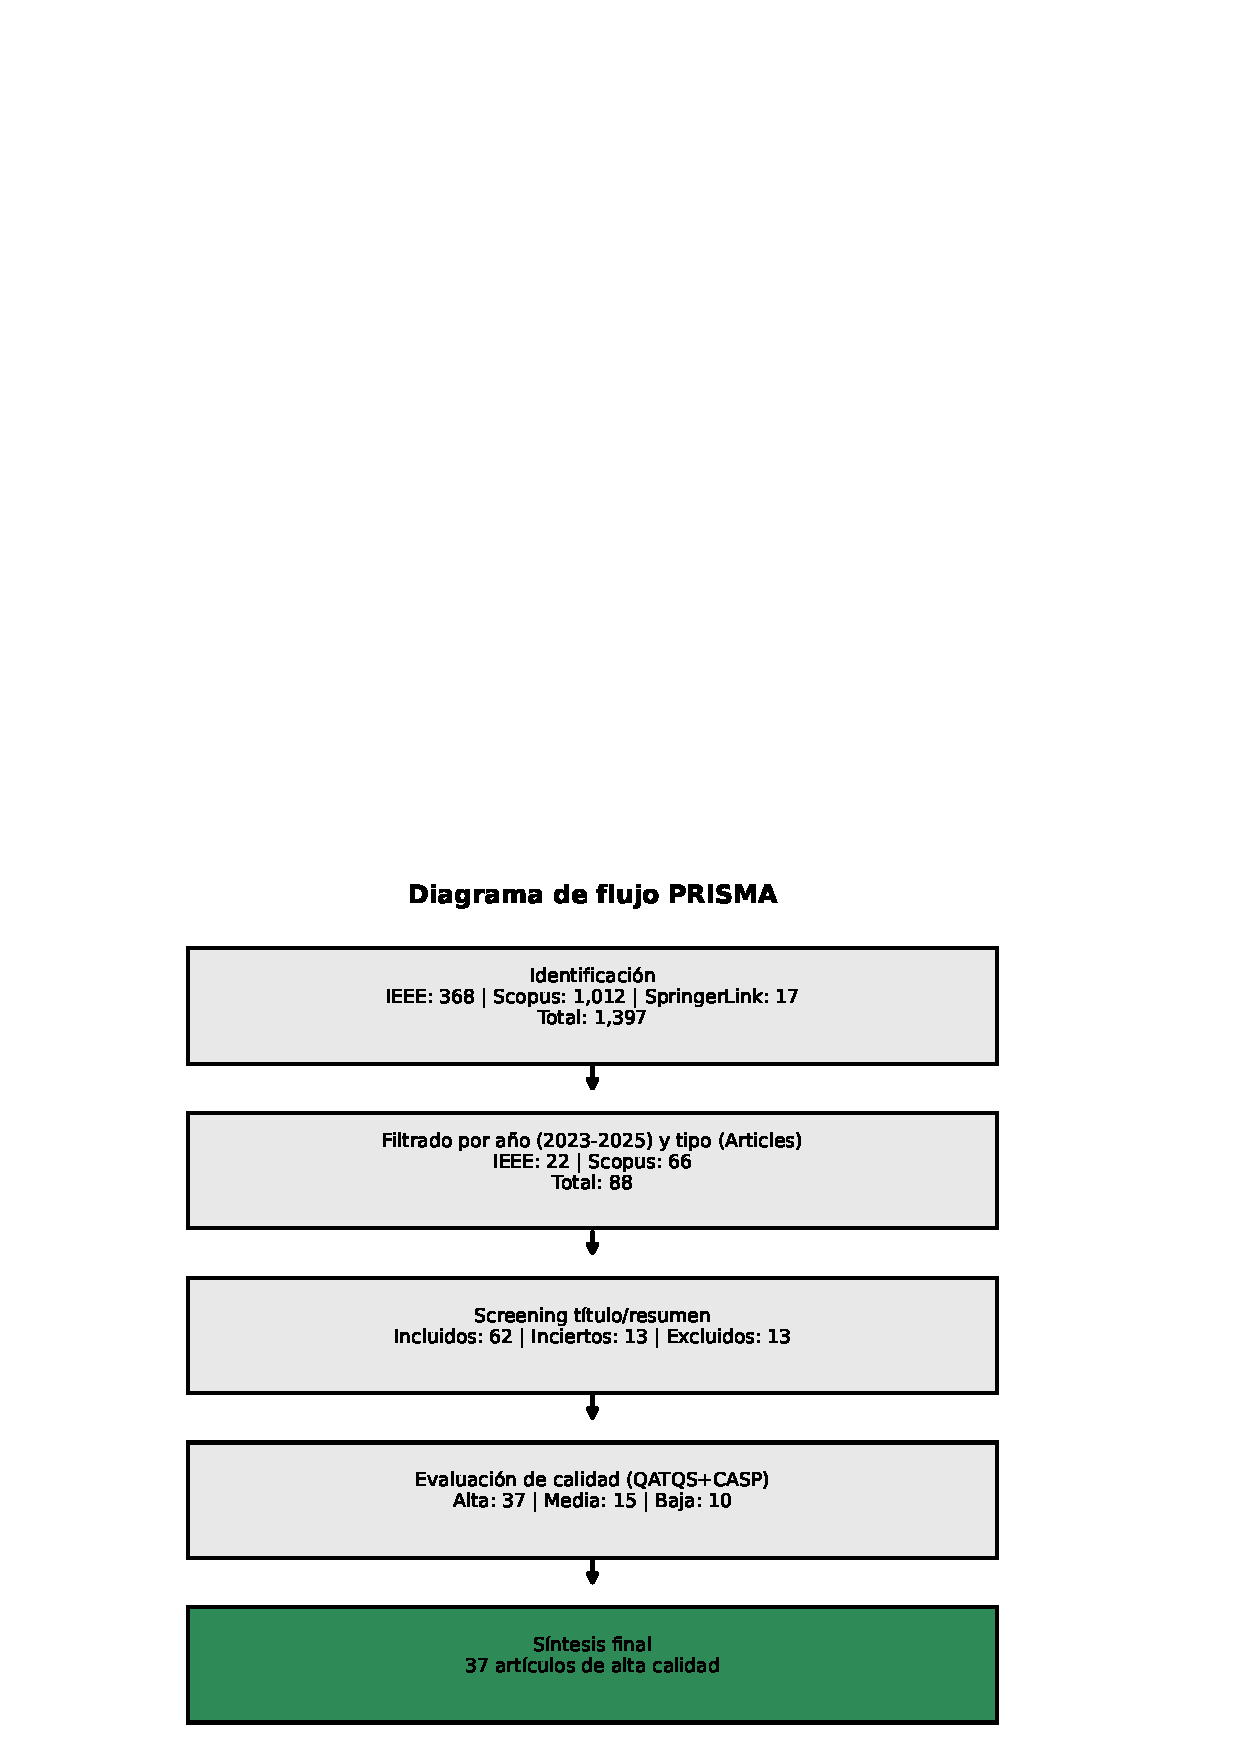
\includegraphics[width=0.85\textwidth]{fig5_prisma.png}
\caption{Diagrama de flujo PRISMA: de 1,397 art\'iculos iniciales a 37 de alta calidad para s\'intesis}
\label{fig:prisma}
\end{figure}

\subsection{Caracter\'isticas de los Estudios Incluidos}

\textbf{Distribuci\'on temporal:} Se observa un crecimiento acelerado en publicaciones: 2023 (n=5, 13.5\%), 2024 (n=14, 37.8\%), 2025 (n=18, 48.7\%). Este patr\'on refleja el inter\'es creciente post-lanzamiento de ChatGPT y herramientas similares.

\textbf{Distribuci\'on geogr\'afica:} Europa lidera con 40.5\% de los estudios, seguida por Am\'ericas (24.3\%), Asia (21.6\%), Ocean\'ia (8.1\%), y otros (5.4\%). La predominancia europea puede explicarse por el marco regulatorio GDPR que impulsa investigaci\'on sobre fairness, privacidad y \'etica en IA.

\textbf{Tipos de estudio:} Experimental (29.7\%), Survey/Cuestionario (21.6\%), Case Study (18.9\%), Mixed Methods (16.2\%), Qualitative/Entrevistas (13.5\%). La diversidad metodol\'ogica permite triangulaci\'on y validaci\'on cruzada de hallazgos.

\textbf{Contexto organizacional:} Corporaciones grandes (37.8\%), Mixto SME/Corporaci\'on (32.4\%), No especificado (29.7\%). Notablemente, pocos estudios se enfocan exclusivamente en SMEs, representando un gap de investigaci\'on.

\begin{figure}[H]
\centering
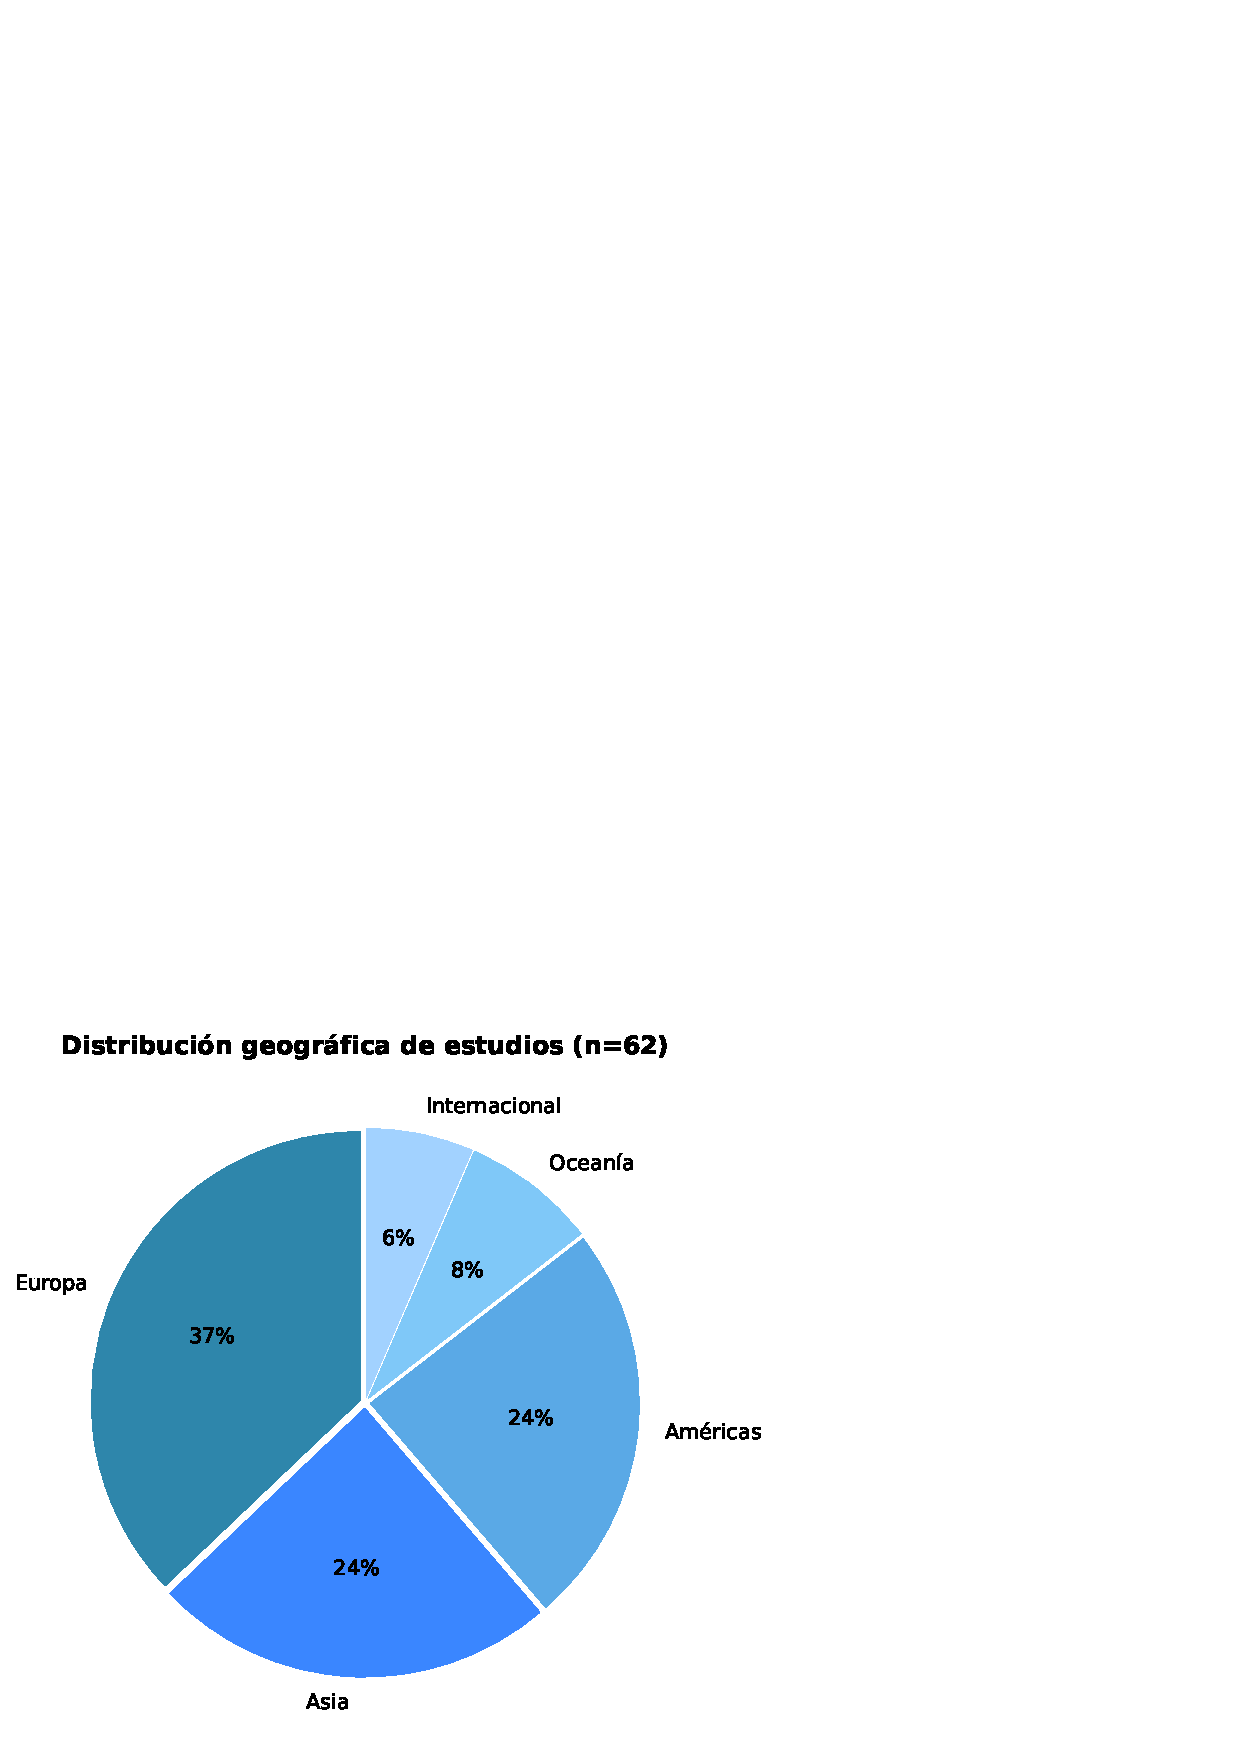
\includegraphics[width=0.75\textwidth]{fig4_geografia.png}
\caption{Distribuci\'on geogr\'afica de los 37 estudios de alta calidad seleccionados}
\label{fig:geografia}
\end{figure}

\subsection{Distribuci\'on de Calidad Metodol\'ogica}

La Tabla~\ref{tab:calidad} presenta la distribuci\'on de calidad por base de datos. Scopus contribuy\'o mayor volumen (50 art\'iculos) con distribuci\'on similar a IEEE en proporciones de calidad.

\begin{table}[H]
\centering
\small
\caption{Distribuci\'on de calidad metodol\'ogica por base de datos}
\label{tab:calidad}
\begin{tabular}{@{}lrrrr@{}}
\toprule
\textbf{Nivel de Calidad} & \textbf{IEEE} & \textbf{Scopus} & \textbf{Total} & \textbf{\%} \\
\midrule
Alta (9-12 puntos) & 9 & 28 & 37 & 59.7 \\
Media (6-8 puntos) & 2 & 13 & 15 & 24.2 \\
Baja ($<$6 puntos) & 1 & 9 & 10 & 16.1 \\
\midrule
\textbf{Total evaluados} & \textbf{12} & \textbf{50} & \textbf{62} & 100 \\
\bottomrule
\end{tabular}
\end{table}

Los tres art\'iculos con puntuaci\'on m\'axima (12 puntos) fueron: Robredo et al.~\cite{robredo2025} (mixed methods con 31 proyectos Java + survey a 23 profesionales), Jiang et al.~\cite{jiang2024} (estudio de reingeniería de modelos DL con triangulaci\'on), y Obie et al.~\cite{obie2023} (detecci\'on de violaciones de honestidad con metodolog\'ia mixta ejemplar).

El criterio con menor cumplimiento fue C9 (reproducibilidad): solo 35.1\% de estudios comparten c\'odigo o datos, reflejando un problema sist\'emico en la disciplina. Los estudios experimentales obtuvieron puntuaciones promedio superiores (media=10.3, DE=1.2) comparados con estudios cualitativos (media=9.1, DE=1.5).

\begin{figure}[H]
\centering
\includegraphics[width=0.75\textwidth]{fig3_calidad_tipo.png}
\caption{Distribuci\'on de puntuaci\'on de calidad por tipo de estudio}
\label{fig:calidad}
\end{figure}

Los tres art\'iculos con puntuaci\'on m\'axima (12 pts) fueron: Robredo et al.~\cite{robredo2025} (mixed methods), Jiang et al.~\cite{jiang2024} (DL reengineering), y Obie et al.~\cite{obie2023} (metodolog\'ia mixta con triangulaci\'on). El criterio con menor cumplimiento fue C9 (reproducibilidad): solo 35.1\% de estudios comparten c\'odigo o datos.

\subsection{S\'intesis por Pregunta de Investigaci\'on}

\textbf{RQ1 - Herramientas de IA/ML adoptadas:} 

La Figura~\ref{fig:herramientas} muestra la distribuci\'on de herramientas. Las t\'ecnicas ML/DL tradicionales dominan con 34\% (n=17), aplicadas principalmente a effort estimation~\cite{rahman2024}, bug triaging~\cite{adhikari2025,hong2024}, y an\'alisis de requirements~\cite{ali2025,izhar2025}. 

ChatGPT representa 28\% (n=14), usado principalmente para code generation, documentaci\'on, y como asistente personal de desarrollo. GitHub Copilot alcanza 24\% (n=9), enfocado en code completion y pair programming asistido. LLMs customizados con arquitecturas RAG representan 11\% (n=7), principalmente en implementaciones enterprise que requieren conocimiento de dominio espec\'ifico~\cite{yang2025}.

Kemell et al.~\cite{kemell2025} reportan un hallazgo cr\'itico: en las 7 organizaciones europeas estudiadas, GenAI se usa principalmente como ``asistentes personales'' sin integraci\'on en workflows organizacionales formales. Esta brecha entre adopci\'on individual y organizacional es un tema recurrente.

\begin{figure}[H]
\centering
\includegraphics[width=0.75\textwidth]{fig1_herramientas.png}
\caption{Distribuci\'on de herramientas IA/ML adoptadas en los estudios analizados}
\label{fig:herramientas}
\end{figure}

\textbf{RQ2 - Factores de \'exito para la adopci\'on:} 

Se identificaron factores agrupados en tres dimensiones:

\textit{Dimensi\'on Tecnol\'ogica:} Automatizaci\'on de tareas repetitivas (n=18, 48.6\%), interfaz intuitiva y baja curva de aprendizaje (n=14, 37.8\%), integraci\'on nativa con pipelines CI/CD (n=11, 29.7\%), calidad consistente de outputs (n=9, 24.3\%), y personalizaci\'on a contexto de dominio (n=8, 21.6\%).

\textit{Dimensi\'on Organizacional:} Cultura de experimentaci\'on y tolerancia al fallo (n=16, 43.2\%), gesti\'on proactiva de expectativas desde el inicio (n=13, 35.1\%), pol\'iticas claras de uso y gobernanza (n=10, 27.0\%), liderazgo visible apoyando iniciativas (n=9, 24.3\%), y m\'etricas de \'exito definidas (n=7, 18.9\%).

\textit{Dimensi\'on Humana:} Capacitaci\'on estructurada y continua (n=15, 40.5\%), awareness expl\'icito de limitaciones de la tecnolog\'ia (n=14, 37.8\%), colaboraci\'on cross-funcional entre equipos (n=12, 32.4\%), champions internos que promueven adopci\'on (n=10, 27.0\%), y comunidades de pr\'actica para compartir experiencias (n=8, 21.6\%).

\textbf{RQ3 - Barreras principales:} 

Las cinco barreras m\'as frecuentemente reportadas son:

(1) \textit{Gesti\'on de expectativas/hype} (56.8\%, n=21): Dolata et al.~\cite{dolata2024} describen c\'omo expectativas infladas por marketing y medios generan ciclos de decepci\'on cuando la tecnolog\'ia no cumple promesas exageradas.

(2) \textit{Calidad de datos} (54.1\%, n=20): Kalinowski et al.~\cite{kalinowski2025}, en su survey internacional con 188 practitioners de 25 pa\'ises, identifican data quality como el ``pain point'' n\'umero uno en sistemas ML-enabled.

(3) \textit{Falsos positivos} (51.4\%, n=19): Stradowski y Madeyski~\cite{stradowski2025}, en su estudio con Nokia 5G, documentan c\'omo desarrolladores pierden confianza en herramientas de IA cuando generan demasiadas alertas incorrectas.

(4) \textit{Alucinaciones de LLMs} (48.6\%, n=18): M\'ultiples estudios reportan que LLMs generan c\'odigo o respuestas plausibles pero incorrectas, requiriendo verificaci\'on humana constante.

(5) \textit{Silos organizacionales} (43.2\%, n=16): V\"ansk\"a et al.~\cite{vanska2024} describen c\'omo la separaci\'on entre equipos de desarrollo, datos y ML dificulta la integraci\'on efectiva de pr\'acticas de IA/ML.

\textbf{RQ4 - Competencias emergentes requeridas:} 

Las competencias m\'as demandadas seg\'un frecuencia de menci\'on son:

(1) Prompt engineering (n=16, 43.2\%): Banh et al.~\cite{banh2025} lo identifican como competencia fundamental, incluyendo t\'ecnicas como chain-of-thought, few-shot learning, y prompt chaining.

(2) Evaluaci\'on cr\'itica de outputs (n=15, 40.5\%): Capacidad de verificar, validar y corregir sugerencias de IA antes de integrarlas.

(3) Fundamentos de ML (n=14, 37.8\%): Comprensi\'on b\'asica de c\'omo funcionan modelos, sus limitaciones y supuestos.

(4) MLOps/DevOps para AI (n=13, 35.1\%): Habilidades para desplegar, monitorear y mantener modelos en producci\'on~\cite{steidl2023,protschky2025}.

(5) Data literacy (n=12, 32.4\%): Capacidad de evaluar calidad de datos, identificar sesgos, y preparar datasets.

(6) Fairness/\'etica en IA (n=11), (7) RE para AI (n=9), (8) Interpretabilidad (n=8).

\textbf{RQ5 - Pr\'acticas emergentes:} Las pr\'acticas identificadas incluyen: AI-Augmented Development (n=18), RAG-based assistants (n=12)~\cite{yang2025}, Fairness-aware ML (n=11)~\cite{ferrara2024,demartino2025}, Continuous AI/ML (n=10)~\cite{vanska2024,steidl2023}, Prompt repositories (n=9), AI code review (n=8)~\cite{alami2025}, Bug triaging automatizado (n=8)~\cite{adhikari2025,hong2024}, ML effort estimation (n=7)~\cite{rahman2024}, AI requirements analysis (n=7)~\cite{ali2025,izhar2025}, y ML observability (n=6)~\cite{protschky2025}.

La Tabla~\ref{tab:rq_resumen} resume los hallazgos principales.

\begin{table}[H]
\centering
\small
\caption{Resumen consolidado de hallazgos por pregunta de investigaci\'on}
\label{tab:rq_resumen}
\begin{tabular}{@{}p{1.2cm}p{3cm}p{4cm}p{4cm}@{}}
\toprule
\textbf{RQ} & \textbf{Foco} & \textbf{Hallazgo Principal} & \textbf{Implicaci\'on} \\
\midrule
RQ1 & Herramientas & ML/DL (34\%), ChatGPT (28\%), Copilot (24\%) & Diversidad tecnol\'ogica requiere estrategias diferenciadas \\
RQ2 & Factores \'exito & Automatizaci\'on + Cultura + Capacitaci\'on & Enfoque tridimensional es cr\'itico \\
RQ3 & Barreras & Hype (57\%), Datos (54\%), FP (51\%) & Barreras humanas superan t\'ecnicas \\
RQ4 & Competencias & Prompt eng. + Evaluaci\'on cr\'itica + ML basics & Nuevos programas formativos requeridos \\
RQ5 & Pr\'acticas & AI-Augmented Dev + RAG + Fairness & Integraci\'on gradual, no disruptiva \\
\bottomrule
\end{tabular}
\end{table}

\subsection{An\'alisis Comparativo SME vs. Corporaciones}

De los 26 estudios que especifican contexto organizacional, se extrajo un an\'alisis comparativo detallado (Tabla~\ref{tab:comparacion}).

\begin{table}[H]
\centering
\small
\caption{An\'alisis comparativo SMEs vs. Corporaciones en adopci\'on de IA/ML}
\label{tab:comparacion}
\begin{tabular}{@{}p{2.8cm}p{4.8cm}p{4.8cm}@{}}
\toprule
\textbf{Dimensi\'on} & \textbf{SMEs} & \textbf{Corporaciones} \\
\midrule
Herramientas preferidas & ChatGPT (67\%), Copilot (44\%), APIs comerciales & LLMs custom con RAG (57\%), plataformas enterprise \\
Barreras principales & Falta de expertise interno (89\%), Budget limitado (78\%), Tiempo de staff (67\%) & Silos organizacionales (79\%), Sistemas legacy (71\%), Compliance (64\%) \\
Motivaci\'on primaria & Bajo costo, r\'apida implementaci\'on, competitividad & Control total, seguridad de datos, compliance regulatorio \\
Modelo de adopci\'on & Bottom-up, impulsado por desarrolladores individuales & Top-down, con governance formal y pilotos estructurados \\
Time-to-value & Semanas a meses & Meses a a\~nos \\
\bottomrule
\end{tabular}
\end{table}

La triangulaci\'on con literatura gris (reportes de GitHub, Stack Overflow, Gartner) muestra alta concordancia en tres temas: (1) alucinaciones de LLMs como barrera cr\'itica, (2) gesti\'on de expectativas como factor de \'exito clave, y (3) prompt engineering como competencia emergente fundamental.

\section{Discusi\'on}

\subsection{Hallazgos Principales y Contribuci\'on Te\'orica}

El hallazgo central de esta RSL es la brecha persistente entre adopci\'on individual y organizacional de IA/ML en desarrollo de software. Mientras 75\% de desarrolladores reportan usar herramientas de IA individualmente, la integraci\'on en workflows organizacionales formales permanece limitada. Kemell et al.~\cite{kemell2025} caracterizan esto elocuentemente como ``still just personal assistants'', indicando que GenAI a\'un no ha trascendido el uso personal hacia workflows organizacionales estructurados.

Este hallazgo tiene implicaciones te\'oricas importantes: sugiere que la adopci\'on de tecnolog\'ias de IA en desarrollo de software sigue un patr\'on diferente a otras tecnolog\'ias, donde la adopci\'on individual precede significativamente a la organizacional. Esto contrasta con tecnolog\'ias anteriores (ej: metodolog\'ias \'agiles, DevOps) donde la adopci\'on fue m\'as frecuentemente top-down.

Dolata et al.~\cite{dolata2024}, en su estudio con 52 freelancers, demuestran que la adopci\'on actual est\'a impulsada mayormente por hype medi\'atico m\'as que por evidencia s\'olida de beneficios, creando ciclos de expectativas infladas seguidas de decepci\'on cuando la tecnolog\'ia no cumple promesas exageradas.

Geogr\'aficamente, Europa lidera la producci\'on de investigaci\'on (40.5\%), posiblemente influenciado por el marco regulatorio GDPR que impulsa estudios sobre fairness, privacidad y \'etica en IA. Esto representa tanto una fortaleza (investigaci\'on m\'as rigurosa sobre aspectos \'eticos) como una limitaci\'on (posible sobre-representaci\'on de contextos regulatorios espec\'ificos).

\subsection{Marco Tridimensional Propuesto}

Basado en la s\'intesis, proponemos un marco de adopci\'on con tres dimensiones interrelacionadas:

\textbf{Dimensi\'on Tecnol\'ogica:} SMEs deben priorizar herramientas comerciales (ChatGPT, Copilot) por bajo costo; corporaciones pueden justificar LLMs custom/RAG para mayor control. Integraci\'on CI/CD, data pipelines y observabilidad son cr\'iticos para escalar.

\textbf{Dimensi\'on Organizacional:} Gesti\'on de expectativas realista, pol\'iticas claras de uso, KPIs medibles, y estructuras que rompan silos entre equipos SE/DS/ML. Evitar ``AI washing'' donde se promueven iniciativas por imagen sin valor real.

\textbf{Dimensi\'on Humana:} Programas de training en prompt engineering/MLOps, cultura de experimentaci\'on con tolerancia al fallo, repositorios de best practices, y desarrollo de evaluaci\'on cr\'itica.

\subsection{Roadmap de Implementaci\'on}

\textbf{Fase 1 - Piloto (3-6 meses):} 1-2 use cases acotados, equipo de early adopters, m\'etricas baseline.

\textbf{Fase 2 - Escalamiento (6-12 meses):} Pol\'iticas formales, training ampliado, integraci\'on CI/CD, repositorios de prompts.

\textbf{Fase 3 - Institucionalizaci\'on (12+ meses):} IA/ML standard en SDLC, MLOps maduro, gobernanza formal.

\subsection{Implicaciones y Limitaciones}

\textbf{Implicaciones pr\'acticas:} Desarrolladores deben invertir en prompt engineering y evaluaci\'on cr\'itica. L\'ideres t\'ecnicos deben fomentar experimentaci\'on controlada y medir impacto real. Organizaciones deben abordar las tres dimensiones simult\'aneamente sin esperar ``silver bullets''.

\textbf{Limitaciones:} (1) Per\'iodo temporal 2023-2025; (2) Exclusi\'on de SpringerLink; (3) Sesgo de publicaci\'on hacia casos exitosos; (4) Sesgo de idioma (ingl\'es/espa\~nol); (5) Evaluaci\'on QATQS+CASP con componente subjetivo; (6) Generalizaci\'on limitada (40.5\% Europa).

\subsection{Agenda de Investigaci\'on Futura}

Se identifican las siguientes direcciones prioritarias para investigaci\'on futura:

\textit{Estudios longitudinales}: Seguimiento de organizaciones 2-3 a\~nos post-adopci\'on para evaluar impacto real y sostenibilidad.

\textit{Modelos de madurez}: Desarrollo de frameworks para evaluar nivel de madurez en adopci\'on de IA/ML en desarrollo de software.

\textit{Frameworks de ROI}: M\'etodos rigurosos para cuantificar retorno de inversi\'on de iniciativas de IA en desarrollo.

\textit{RCTs comparativos}: Experimentos controlados comparando efectividad de diferentes herramientas y enfoques.

\textit{Curr\'icula educativa}: Desarrollo y validaci\'on de programas de formaci\'on en prompt engineering y MLOps.

\textit{Fairness y \'etica}: Mayor investigaci\'on sobre pr\'acticas de IA responsable en contextos de desarrollo de software.

\textit{Contextos sub-representados}: Estudios espec\'ificos en regiones como \'Africa, Latinoam\'erica y Asia emergente.

\section{Conclusiones}

Esta revisi\'on sistem\'atica de literatura sintetiz\'o 37 estudios de alta calidad metodol\'ogica (de 1,397 iniciales) sobre adopci\'on de IA/ML en desarrollo de software empresarial durante el per\'iodo 2023-2025, siguiendo rigurosamente las directrices de Kitchenham y el protocolo PRISMA.

\textbf{RQ1 - Herramientas:} ChatGPT (28\%), GitHub Copilot (24\%) y t\'ecnicas ML/DL tradicionales (34\%) dominan el panorama. Existe clara diferenciaci\'on por contexto: SMEs prefieren herramientas comerciales de bajo costo; corporaciones desarrollan LLMs customizados con RAG (57\%) para mayor control y seguridad.

\textbf{RQ2 - Factores de \'exito:} La tr\'iada tecnolog\'ia-organizaci\'on-humano es cr\'itica. Los factores m\'as frecuentes son automatizaci\'on de tareas repetitivas (n=18), cultura de experimentaci\'on (n=16), y capacitaci\'on estructurada (n=15). El \'exito requiere abordar las tres dimensiones simult\'aneamente.

\textbf{RQ3 - Barreras:} Las cinco barreras principales son gesti\'on de expectativas/hype (56.8\%), calidad de datos (54.1\%), falsos positivos (51.4\%), alucinaciones de LLMs (48.6\%), y silos organizacionales (43.2\%). Notablemente, las barreras humanas y organizacionales superan a las t\'ecnicas.

\textbf{RQ4 - Competencias:} Las competencias emergentes clave son prompt engineering (n=16), evaluaci\'on cr\'itica de outputs (n=15), fundamentos de ML (n=14), y MLOps (n=13). Estas competencias requieren programas de formaci\'on espec\'ificos a\'un poco maduros en la industria.

\textbf{RQ5 - Pr\'acticas:} Las pr\'acticas emergentes m\'as frecuentes son AI-Augmented Development (n=18), RAG-based assistants (n=12), fairness-aware ML (n=11), y continuous AI/ML integration (n=10). Estas pr\'acticas representan la vanguardia de la integraci\'on de IA en desarrollo de software.

\textbf{Contribuciones principales:} Este trabajo aporta: (1) marco tridimensional integrado para comprender adopci\'on de IA/ML, (2) taxonom\'ia actualizada de herramientas y pr\'acticas, (3) an\'alisis comparativo detallado SME vs. corporaciones, (4) roadmap faseado para implementaci\'on, y (5) triangulaci\'on validada con literatura gris industrial.

\textbf{Mensaje clave:} La adopci\'on individual de IA en desarrollo de software es alta (75\%), pero la integraci\'on organizacional permanece significativamente limitada. El \'exito sostenible requiere un enfoque hol\'istico que combine tecnolog\'ia adecuada, transformaci\'on organizacional, y desarrollo de competencias humanas, con gesti\'on de expectativas realista e inversi\'on sostenida en capacitaci\'on. No existe \textit{silver bullet}: las estrategias deben contextualizarse cuidadosamente seg\'un tama\~no organizacional, madurez tecnol\'ogica y capacidades existentes.

\begin{thebibliography}{30}
\bibitem{kitchenham2007} Kitchenham, B., Charters, S.: Guidelines for performing systematic literature reviews in software engineering. Keele University and Durham University, EBSE Technical Report (2007)

\bibitem{kemell2025} Kemell, K.K., Saarikallio, M., Nguyen-Duc, A., Abrahamsson, P.: Still just personal assistants? -- A multiple case study of generative AI adoption in software organizations. Inf. Softw. Technol. \textbf{186}, 107805 (2025). \url{https://doi.org/10.1016/j.infsof.2025.107805}

\bibitem{dolata2024} Dolata, M., Lange, N., Schwabe, G.: Development in Times of Hype: How Freelancers Explore Generative AI? In: Proc. IEEE/ACM ICSE, pp. 2257--2269 (2024). \url{https://doi.org/10.1145/3597503.3639111}

\bibitem{kalinowski2025} Kalinowski, M., Mendez, D., Giray, G., et al.: Naming the Pain in machine learning-enabled systems engineering. Inf. Softw. Technol. \textbf{187}, 107866 (2025). \url{https://doi.org/10.1016/j.infsof.2025.107866}

\bibitem{banh2025} Banh, L., Holldack, F., Strobel, G.: Copiloting the future: How generative AI transforms Software Engineering. Inf. Softw. Technol. \textbf{183}, 107751 (2025). \url{https://doi.org/10.1016/j.infsof.2025.107751}

\bibitem{ferrara2024} Ferrara, C., Sellitto, G., Ferrucci, F., Palomba, F., De Lucia, A.: Fairness-aware machine learning engineering: how far are we? Empir. Softw. Eng. \textbf{29}(1), 27 (2024). \url{https://doi.org/10.1007/s10664-023-10402-y}

\bibitem{stradowski2025} Stradowski, S., Madeyski, L.: Your AI is impressive, but my code does not have any bugs: managing false positives in industrial contexts. Sci. Comput. Program. \textbf{246}, 103320 (2025). \url{https://doi.org/10.1016/j.scico.2025.103320}

\bibitem{jensen2025} Jensen, V.V., Alami, A., Bruun, A.R., Persson, J.S.: Managing expectations towards AI tools for software development: a multiple-case study. Inf. Syst. e-Bus. Manag. (2025). \url{https://doi.org/10.1007/s10257-025-00704-7}

\bibitem{yang2025} Yang, R., Fu, M., Tantithamthavorn, K., et al.: RAGVA: Engineering retrieval augmented generation-based virtual assistants in practice. J. Syst. Softw. \textbf{226}, 112436 (2025). \url{https://doi.org/10.1016/j.jss.2025.112436}

\bibitem{vanska2024} V\"ansk\"a, S., Kemell, K.K., Mikkonen, T., Abrahamsson, P.: Continuous Software Engineering Practices in AI/ML Development Past the Narrow Lens of MLOps. e-Informatica Softw. Eng. J. \textbf{18}(1), 240102 (2024). \url{https://doi.org/10.37190/e-Inf240102}

\bibitem{alami2025} Alami, A., Jensen, V.V., Ernst, N.A.: Accountability in Code Review: The Role of Intrinsic Drivers and the Impact of LLMs. ACM Trans. Softw. Eng. Methodol. \textbf{34}(8), 201 (2025). \url{https://doi.org/10.1145/3721127}

\bibitem{steidl2023} Steidl, M., Felderer, M., Ramler, R.: The pipeline for the continuous development of artificial intelligence models -- Current state of research and practice. J. Syst. Softw. \textbf{199}, 111615 (2023). \url{https://doi.org/10.1016/j.jss.2023.111615}

\bibitem{rahman2023} Rahman, M.S., Khomh, F., Hamidi, A., et al.: Machine learning application development: practitioners' insights. Softw. Qual. J. \textbf{31}(4), 1065--1119 (2023). \url{https://doi.org/10.1007/s11219-023-09621-9}

\bibitem{haldar2025} Haldar, S., Pierce, M., Capretz, L.F.: Exploring the Integration of Generative AI Tools in Software Testing Education. IEEE Access \textbf{13}, 46070--46090 (2025). \url{https://doi.org/10.1109/ACCESS.2025.3545882}

\bibitem{baralla2024} Baralla, G., Ibba, G., Tonelli, R.: Assessing GitHub Copilot in Solidity Development: Capabilities, Testing, and Bug Fixing. IEEE Access \textbf{12}, 164389--164411 (2024). \url{https://doi.org/10.1109/ACCESS.2024.3486365}

\bibitem{rahman2024} Rahman, M., Sarwar, H., Kader, M.A., Gon\c{c}alves, T., Tin, T.: Review and Empirical Analysis of Machine Learning-Based Software Effort Estimation. IEEE Access \textbf{12}, 85661--85680 (2024). \url{https://doi.org/10.1109/ACCESS.2024.3404879}

\bibitem{adhikari2025} Adhikari, N., Bista, R., Ferreira, J.C.: Leveraging Machine Learning for Enhanced Bug Triaging in Open-Source Software Projects. IEEE Access \textbf{13}, 136237--136254 (2025). \url{https://doi.org/10.1109/ACCESS.2025.3595011}

\bibitem{ali2025} Ali, H., Tanveer, U., Saeed, A., et al.: Cloud-based machine learning for scalable classification of software requirements. Syst. Soft Comput. \textbf{7}, 200405 (2025). \url{https://doi.org/10.1016/j.sasc.2025.200405}

\bibitem{robredo2025} Robredo, M., Saarim\"aki, N., Esposito, M., Taibi, D., et al.: Evaluating time-dependent methods in code technical debt prediction. J. Syst. Softw. \textbf{230}, 112545 (2025). \url{https://doi.org/10.1016/j.jss.2025.112545}

\bibitem{izhar2025} Izhar, R., Bhatti, S.N., Alharthi, S.A.: A Novel Machine Learning Approach for Ambiguity Detection in Software Requirements. IEEE Access \textbf{13}, 12014--12031 (2025). \url{https://doi.org/10.1109/ACCESS.2025.3529943}

\bibitem{russo2024} Russo, D.: Navigating the Complexity of Generative AI Adoption in Software Engineering. ACM Trans. Softw. Eng. Methodol. \textbf{33}(5), 123 (2024). \url{https://doi.org/10.1145/3652154}

\bibitem{eramo2024} Eramo, R., Said, B., Oriol, M., Bruneli\`ere, H., Morales, S.: An architecture for model-based and intelligent automation in DevOps. J. Syst. Softw. \textbf{217}, 112180 (2024). \url{https://doi.org/10.1016/j.jss.2024.112180}

\bibitem{duda2024} Duda, S., Hofmann, P., Urbach, N., V\"olter, F., Zwickel, A.: The Impact of Resource Allocation on the Machine Learning Lifecycle. Bus. Inf. Syst. Eng. \textbf{66}(2), 203--219 (2024). \url{https://doi.org/10.1007/s12599-023-00842-7}

\bibitem{jiang2024} Jiang, W., Banna, V., Vivek, N., et al.: Challenges and practices of deep learning model reengineering: A case study on computer vision. Empir. Softw. Eng. \textbf{29}(6), 144 (2024). \url{https://doi.org/10.1007/s10664-024-10521-0}

\bibitem{obie2023} Obie, H.O., Du, H., Madampe, K., et al.: Automated detection, categorisation and developers' experience with the violations of honesty in mobile apps. Empir. Softw. Eng. \textbf{28}(6), 145 (2023). \url{https://doi.org/10.1007/s10664-023-10361-4}

\bibitem{hong2024} Hong, H.T., Wang, D., Kim, S., et al.: Implementing and Evaluating Automated Bug Triage in Industrial Projects. IEEE Access \textbf{12}, 193717--193730 (2024). \url{https://doi.org/10.1109/ACCESS.2024.3519418}

\bibitem{protschky2025} Protschky, D., Lammermann, L., Hofmann, P., Urbach, N.: What Gets Measured Gets Improved: Monitoring Machine Learning Applications. IEEE Access \textbf{13}, 34518--34538 (2025). \url{https://doi.org/10.1109/ACCESS.2025.3534628}

\bibitem{quaranta2025} Quaranta, L., Azevedo, K., Calefato, F., Kalinowski, M.: A multivocal literature review on the benefits and limitations of AutoML tools. Inf. Softw. Technol. \textbf{178}, 107608 (2025). \url{https://doi.org/10.1016/j.infsof.2024.107608}

\bibitem{demartino2025} De Martino, V., Voria, G., Troiano, C., et al.: Examining the impact of bias mitigation algorithms on ML-enabled systems sustainability. J. Syst. Softw. \textbf{230}, 112458 (2025). \url{https://doi.org/10.1016/j.jss.2025.112458}

\bibitem{github2024} GitHub: The Economic Impact of the AI-Powered Developer Lifecycle. GitHub Research Report (2024). \url{https://github.blog/news-insights/research/}
\end{thebibliography}

\end{document}
